\begin{comment}

TODO: Data exploration
TODO: Data pre-processing
TODO: Dealing with missing data
TODO: Moving average smoothing
TODO: Results

\end{comment}

An essential step between acquiring of the data and passing it to machine learning algorithms is ensuring that the dataset used for training represents our learning objectives. In this case, our learning objective is to train the system to recognize two of the well-known gymnastics movements - the backflip and the back handspring. A well-balanced and interpretable dataset is necessary for avoiding overfitting or biasing the machine learning model to a specific dataset. 

In the section \ref{data-exploration}, we start by sampling the data and visualizing it to better understand the pose estimation results obtained in the previous chapter. Then, based on the observations, pre-processing strategies for overcoming the shortcomings of the dataset are proposed by the author in section \ref{data-pre-processing-strategies} and lastly the final dataset, ready to be used for machine learning, is described in the \ref{pre-processing-results} section of this chapter.

\section{Data exploration}
\label{data-exploration}

\begin{figure}[htb]
  \centering
    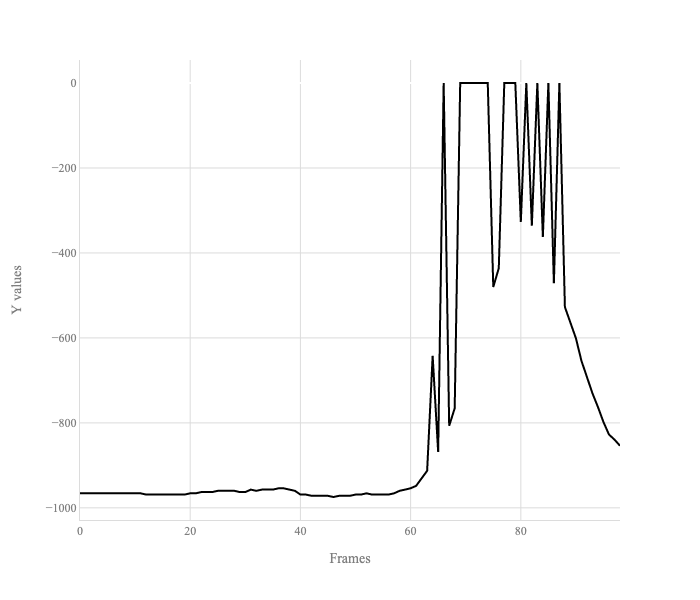
\includegraphics[width=14cm]
    {images/data-preprocessing/flack-17-rasmus-l-heel-y-raw}
    \caption{JSON to Drawing Entity Conversion --- Flow Diagram}
    \label{alg-drawing}
\end{figure}

\section{Data pre-processing strategies}
\label{data-pre-processing-strategies}

\subsection{Dealing with low confidence keypoints}

\subsection{Moving average smoothing}

\subsection{Unrecognizable body parts}

\subsection{Considerations for bystanders}

\section{Results}
\label{pre-processing-results}



